\chapter{Separabilidad}

Previo a definir un espacio métrico separable, veamos qué es la topología de un espacio.

\section{Topología del espacio}

\begin{definition}
	Sea $(X, d)$ un espacio métrico. La \emph{topología} de $X$ es la familia de subconjuntos abiertos de $X$. Una \emph{base} de la topología de $X$ es una familia de abiertos $\mathcal{B}$ tal que
	\begin{center}
		\begin{minipage}{0.9\linewidth}
			todo abierto $A \subseteq X$ se puede expresar como $A = \bigcup_{i \in I} B_i$ con $B_i \in \mathcal{B}$.
		\end{minipage}
	\end{center}
\end{definition}
\begin{remark}
	La condición de una base puede ser reemplazada por:
	\begin{center}
		\begin{minipage}{0.9\linewidth}
			Para todo $A \subseteq X$ abierto se cumple que para todo $a \in A$, existe $B \in \mathcal{B}$ tal que $a \in B \subseteq A$.
		\end{minipage}
	\end{center}
\end{remark}

\begin{example}
	Algunas bases son:
	\begin{enumerate}
		\item La base $\{ B(x, r) \mid x \in X \text{ y } r > 0 \}$.
		\item La familia de abiertos es una base.
		\item La base $\{ B(x, \frac{1}{n}) \mid x \in X \text{ y } n \in \mathbb{N} \}$.
	\end{enumerate}
\end{example}

\begin{definition}
	Decimos que dos espacios métricos tienen \emph{topologías equivalentes} si inducen los mismos abiertos.
\end{definition}

\begin{example}
	En $\mathbb{R}^n$, las métricas $\lVert \cdot \rVert_p$ donde $p \in (0, + \infty]$ inducen la misma topología.
\end{example}

Recordemos la definición de subespacio métrico: subconjunto del espacio con la métrica restringida.

\begin{remark}
	Definimos la bola en $Y \subseteq X$ como
	$$
		B_Y (y, r) = \{ x \in Y \mid d(x, y) < r\}.
	$$
\end{remark}

\begin{proposition}
	Sea $(X, d)$ un espacio métrico e $Y \subseteq X$. Entonces, un subconjunto $A \subseteq Y$ es abierto en $Y$ si y sólo si existe un subconjunto abierto $B \subseteq X$ tal que $A = B \cap Y$.
\end{proposition}

\begin{proof}
	($\Rightarrow$) Sea $A \subseteq Y$ un subconjunto abierto. Entonces, $A$ es unión de bolas abiertas
	$$
		A = \bigcup_{i \in I} B_Y (y_i, r_i).
	$$
	Definimos al conjunto
	$$
		B = \bigcup_{i \in I} B (y_i, r_i).
	$$
	Dado que $B$ es unión de abiertos,  también es abierto. Consideramos
	$$
		B \cap Y = \bigcup_{i \in I} B_Y (y_i, r_i) = A.
	$$

	($\Leftarrow$) Sea $A \subseteq Y$ y $B \subseteq X$ un subconjunto abierto que cumplen que $A = B \cap Y$. Como $B$ es abierto, se puede expresar como la unión de bolas abiertas
	$$
		B = \bigcup_{i \in I} B(x_i, r_i).
	$$
	Por lo tanto,
	$$
		A = B \cap Y = \bigcup_{i \in I} B_Y (x_i, r_i).
	$$
	Y como $A$ es unión de bolas abiertas, $A$ es abierto.
\end{proof}

\begin{remark}
	La proposición análoga para cerrados también es válida.
\end{remark}

\section{Espacios separables}

\begin{definition}
	Un espacio métrico $(X, d)$ es \emph{separable} si existe un subconjunto denso $D \subseteq X$ tal que $\left| D \right| \leq \aleph_0$.
\end{definition}

\begin{example}
	Algunos espacios separables son:
	\begin{enumerate}
		\item $X$ contable es separable con $D = X$.
		\item $(\mathbb{R}, |\cdot|)$ es separable con $D = \mathbb{Q}$.
		\item $(\mathbb{R} - \mathbb{Q}, |\cdot|)$ es separable con $D = \mathbb{Q} + \sqrt{2}$.
		\item $(\ell^{p} (\mathbb{R}), \lVert \cdot \rVert)$ es separable para $p < + \infty$.
		\item $C([a, b], \mathbb{R})$ es separable con $D = \mathbb{Q}[x]$.
	\end{enumerate}
\end{example}

\begin{definition}
	\begin{itemize}
		\item Decimos que una familia $\{ A_i \}_{i \in I}$ es un \emph{cubrimiento} de $X$ si $X \subseteq \bigcup_{i \in I} A_i$.
		\item Si además $B_i$ es abierto para todo $i \in I$, decimos que $\{ B_i \}_{i \in I}$ es un \emph{cubrimiento abierto} de $X$.
		\item La familia $\{ A_j \}_{j \in J}$ es un \emph{subcubrimiento} de $\{ A_i \}_{i \in I}$ si es un cubrimiento y $J \subseteq I$.
	\end{itemize}
\end{definition}

A continuación enunciamos y demostramos el Teorema de Lindelöf.

\begin{theorem}
	Sea $(X, d)$ un espacio métrico. Entonces, son equivalentes:
	\begin{enumerate}
		\item $X$ es separable.
		\item Existe una base contable de $X$.
		\item Todo cubrimiento abierto de $X$ admite un subcubrimiento contable.
	\end{enumerate}
\end{theorem}

\begin{proof}
	\framebox{1. $\Rightarrow$ 2.} Sea $(X, d)$ un espacio métrico separable. Entonces, existe un subconjunto denso $D \subseteq X$ contable. Veamos que
	$$
		\mathcal{B} = \left\{ B\left(x, \frac{1}{n}\right) \right\}_{x \in D, n \in \mathbb{N}}
	$$
	es una base contable. Dado que $D \times \mathbb{N}$ es contable, $\mathcal{B}$ es contable, basta con ver que para todo $A \subseteq X$ abierto y todo $a \in A$, existe $B \in \mathcal{B}$ tal que $a \in B \subseteq A$.

	Sea $A \subseteq X$ un subconjunto abierto y sea $a \in A$. Por definición de abierto, existe una bola $B(a, r)$ con $r > 0$ tal que $B(a, r) \subseteq A$. Queremos encontrar $x \in D$ y $r' > 0$ tales que $a \in B(x, r') \subseteq B(a, r)$. Elegimos $r' = \frac{1}{n}$ tal que $\frac{1}{n} < \frac{r}{2}$. Consideramos ahora la bola $B(a, \frac{1}{n})$. Dado que $D$ es denso, existe $x \in D$ tal que $x \in B(a, \frac{1}{n})$.

	Veamos que $a \in B(x, \frac{1}{n}) \subseteq B(a, r)$. Sea $x' \in B(x, \frac{1}{n})$. Entonces,
	$$
		d(x', a) \leq d(x', x) + d(x, a) < \frac{2}{n} < r.
	$$
	\begin{center}
		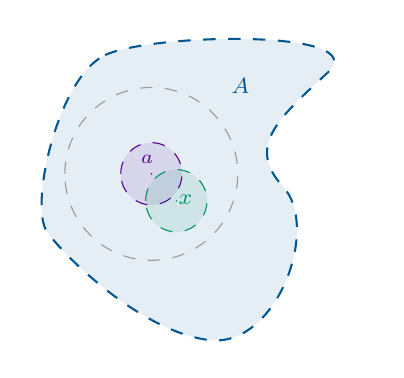
\begin{tikzpicture}[x=0.75pt,y=0.75pt,yscale=-1,xscale=1]
	%uncomment if require: \path (0,300); %set diagram left start at 0, and has height of 300

	%Shape: Polygon Curved [id:ds7613739725483922] 
	\draw  [color={rgb, 255:red, 0; green, 86; blue, 145 }  ,draw opacity=1 ][fill={rgb, 255:red, 0; green, 86; blue, 145 }  ,fill opacity=0.1 ][dash pattern={on 4.5pt off 4.5pt}][line width=0.75]  (57.97,34.79) .. controls (80.65,24.22) and (187.88,22.11) .. (165.2,43.24) .. controls (143.21,63.73) and (126.42,77.59) .. (142.1,96.4) .. controls (142.59,96.98) and (143.1,97.57) .. (143.66,98.17) .. controls (161.93,117.89) and (140.5,176.33) .. (107.87,172.11) .. controls (75.24,167.89) and (38.86,132.38) .. (30,120) .. controls (21.14,107.62) and (35.29,45.35) .. (57.97,34.79) -- cycle ;
	%Shape: Ellipse [id:dp42634731485483457] 
	\draw  [color={rgb, 255:red, 86; green, 0; blue, 145 }  ,draw opacity=1 ][fill={rgb, 255:red, 86; green, 0; blue, 145 }  ,fill opacity=0.1 ][dash pattern={on 4.5pt off 4.5pt}] (65.5,92) .. controls (65.5,83.72) and (72.1,77) .. (80.25,77) .. controls (88.4,77) and (95,83.72) .. (95,92) .. controls (95,100.28) and (88.4,107) .. (80.25,107) .. controls (72.1,107) and (65.5,100.28) .. (65.5,92) -- cycle ;
	%Shape: Ellipse [id:dp1598998823581017] 
	\draw  [color={rgb, 255:red, 86; green, 0; blue, 145 }  ,draw opacity=1 ][dash pattern={on 4.5pt off 4.5pt}] (80.2,92.05) .. controls (80.2,92.02) and (80.22,92) .. (80.25,92) .. controls (80.28,92) and (80.3,92.02) .. (80.3,92.05) .. controls (80.3,92.08) and (80.28,92.1) .. (80.25,92.1) .. controls (80.22,92.1) and (80.2,92.08) .. (80.2,92.05) -- cycle ;

	%Shape: Ellipse [id:dp6929882431707403] 
	\draw  [color={rgb, 255:red, 0; green, 145; blue, 105 }  ,draw opacity=1 ][fill={rgb, 255:red, 0; green, 145; blue, 105 }  ,fill opacity=0.1 ][dash pattern={on 4.5pt off 4.5pt}] (77.5,105) .. controls (77.5,96.72) and (84.1,90) .. (92.25,90) .. controls (100.4,90) and (107,96.72) .. (107,105) .. controls (107,113.28) and (100.4,120) .. (92.25,120) .. controls (84.1,120) and (77.5,113.28) .. (77.5,105) -- cycle ;
	%Shape: Ellipse [id:dp7063709012266387] 
	\draw  [color={rgb, 255:red, 0; green, 145; blue, 105 }  ,draw opacity=1 ][fill={rgb, 255:red, 0; green, 145; blue, 105 }  ,fill opacity=0.1 ][dash pattern={on 4.5pt off 4.5pt}] (92.2,105.05) .. controls (92.2,105.02) and (92.22,105) .. (92.25,105) .. controls (92.28,105) and (92.3,105.02) .. (92.3,105.05) .. controls (92.3,105.08) and (92.28,105.1) .. (92.25,105.1) .. controls (92.22,105.1) and (92.2,105.08) .. (92.2,105.05) -- cycle ;

	%Shape: Circle [id:dp3999102181776214] 
	\draw  [color={rgb, 255:red, 155; green, 155; blue, 155 }  ,draw opacity=1 ][dash pattern={on 4.5pt off 4.5pt}] (38.55,92.05) .. controls (38.55,69.05) and (57.2,50.4) .. (80.2,50.4) .. controls (103.2,50.4) and (121.85,69.05) .. (121.85,92.05) .. controls (121.85,115.05) and (103.2,133.7) .. (80.2,133.7) .. controls (57.2,133.7) and (38.55,115.05) .. (38.55,92.05) -- cycle ;

	% Text Node
	\draw (117.65,44.65) node [anchor=north west][inner sep=0.75pt]  [font=\footnotesize,color={rgb, 255:red, 0; green, 86; blue, 145 }  ,opacity=1 ]  {$A$};
	% Text Node
	\draw (74,82) node [anchor=north west][inner sep=0.75pt]  [font=\scriptsize,color={rgb, 255:red, 86; green, 0; blue, 145 }  ,opacity=1 ]  {$a$};
	% Text Node
	\draw (92.25,101) node [anchor=north west][inner sep=0.75pt]  [font=\footnotesize,color={rgb, 255:red, 0; green, 145; blue, 105 }  ,opacity=1 ]  {$x$};

\end{tikzpicture}

	\end{center}

	\framebox{2. $\Rightarrow$ 3.} Sea $\mathcal{B} = \{ B_n \}_{n \in N}$ una base contable de $X$ y sea $\mathcal{U} = \{ U_i \}_{i \in I}$ un cubrimiento abierto. Definimos la función
	\begin{align*}
		\Phi: N & \to I                                         \\
		n       & \mapsto i \text{ tal que } B_n \subseteq U_i.
	\end{align*}
	Y consideramos $J = \operatorname{Im} \Phi$. Seguro que $J$ es contable ya que $\Phi$ es sobreyectiva hacia $J$. Entonces, basta con ver que el subconjunto $\mathcal{U}' = \{ U_j \}_{j \in J}$ cubre a $X$.

	Sea $x \in X$. Como $\mathcal{B}$ es una base, existe algún $n \in N$ tal que $x \in B_n$. Consideramos $j \in J$ tal que $B_n \subseteq U_j$, entonces $x \in U_j$. Por lo tanto, para todo $x \in X$, existe un $j \in J$ tal que $x \in U_j$. Por lo tanto, $\mathcal{U}'$ cubre a $X$.

	\framebox{3. $\Rightarrow$ 1.} Sea $\mathcal{U}_n = \{ B(x, \frac{1}{n}) \mid x \in X\}$. Como $\mathcal{U}_n$ es un cubrimiento abierto, existe un subcubrimiento contable
	$$
		\mathcal{U}'_n = \{ B\left(x, \frac{1}{n}\right) \mid x \in D_n \subseteq X\}.
	$$
	Dado que $\mathcal{U}'_n$ es contable, $D_n$ tiene que serlo también. Sea $D = \bigcup_{n \in \mathbb{N}} D_n$. Veamos que $D$ es denso en $X$.

	Sea $x \in X$ y $r > 0$. Queremos ver que $B(x, r) \cap D \neq \emptyset$. Por Arquimedianidad, existe $N \in \mathbb{N}$ tal que $\frac{1}{N} < r$. Dado que $U'_N$ es un cubrimiento, existe $a \in D_N$ tal que $x \in B(a, \frac{1}{N})$. Entonces, $d(x, a) < \frac{1}{N} < r$. Entonces, $B(x, r) \cap D \neq \emptyset$.
\end{proof}

\begin{corollary}
	Sea $(X, d)$ un espacio métrico separable y sea $Y \subseteq X$ un subespacio. Entonces, $Y$ es separable.
\end{corollary}

\begin{proof}
	Por el Teorema anterior, $(X, d)$ es separable si y sólo si existe una base contable de $X$. Basta con ver que $Y$ tiene una base contable. Consideramos $\mathcal{B}|_Y = \{ B_n \cap Y\}_{n \in \mathbb{N}}$. Esto define una base contable de $Y$.
\end{proof}

\begin{proposition}
	Un espacio métrico $(X, d)$ es separable si y sólo si toda familia de disjuntos abiertos de $X$ es contable.
\end{proposition}

\begin{proof}
	($\Rightarrow$) Sea $(X, d)$ un espacio métrico separable. Sea $\mathcal{U} = \{ U_i \}_{i \in I}$ una familia de disjuntos abiertos de $X$. Por el Teorema anterior, existe una base contable $\mathcal{B}$. Definimos la función
	\begin{align*}
		\varphi: I & \to  N                                         \\
		i          & \mapsto n \text{ tal que } B_n \subseteq U_i .
	\end{align*}
	La función está bien definida ya que, dado que $\mathcal{B}$ es una base, todo elemento de $\mathcal{U}$ se puede expresar como unión de elementos de $\mathcal{B}$ (para la elección podemos simplemente tomar el mínimo de los $n$). Veamos que $\varphi$ es inyectiva. Sean $i, j \in I$ tales que $\varphi(i) = \varphi(j) = n$. Entonces, $B_n \subseteq U_i \cap  U_j$, lo cual es absurdo. Por lo tanto, $\varphi$ es inyectiva.

	Como $\left| N \right| \leq \aleph_0$ y $\left| I \right| \leq \left| N \right| $, obtenemos que $\left| I \right| \leq \aleph_0$, es decir, $I$ es contable.

	($\Leftarrow$) Sea $\mathcal{F}_n$ una familia disjunta de bolas abiertas de radio $\frac{1}{n}$ maximal. Es decir, toda bola de radio $\frac{1}{n}$ interseca con algún elemento de $\mathcal{F}_n$. Por hipótesis, $\mathcal{F}_n$ es contable. Definimos $D_n$ como el conjunto de centros de las bolas de $\mathcal{F}_n$.

	Sea $D = \bigcup_{n \in \mathbb{N}} D_n$. Veamos que $D$ es denso en $X$. Sea $x \in X$, $r > 0$. Basta con ver que $B(x, r) \cap D \neq \emptyset$. Sea $n \in \mathbb{N}$ tal que $\frac{1}{n} < \frac{r}{2}$.

	Supongamos que $B(x, r) \cap D = \emptyset$. Entonces, $B(x, r) \cap D_n = \emptyset$. Notemos que dos bolas cualesquiera se intersecan si y sólo si la distancia entre sus centros es menor a la suma de sus radios.

	Teniendo esto en cuenta, consideremos la bola $B(x, \frac{1}{n})$. Dado que $(x, r) \cap D_n = \emptyset$, seguro que $d(x, a) > r$. Pero como $r > \frac{2}{n}$, entonces $d(x, a) > \frac{1}{n} + \frac{1}{n}$. Por lo que $B(x, \frac{1}{n})$ no interseca con ningún elemento de $\mathcal{F}_n$. Esto es absurdo; por lo tanto, $B(x, r) \cap D \neq \emptyset$. Entonces, $D$ es denso en $X$.
\end{proof}


